\chapter{Ordenamiento}

\index{ordenamiento}

El \key{ordenamiento}
es un problema fundamental del diseño de algoritmos.
Muchos algoritmos eficientes
usan el ordenamiento como subrutina,
porque a menudo es más fácil procesar
los datos si los elementos están en orden.

Por ejemplo, el problema ''¿un arreglo contiene
dos elementos iguales?'' es fácil de resolver usando ordenamiento.
Si el arreglo contiene dos elementos iguales,
quedarán uno junto al otro después de ordenar,
así que es fácil encontrarlos.
De igual forma, el problema ''¿cuál es el elemento más frecuente
de un arreglo?'' puede resolverse de manera similar.

Hay muchos algoritmos de ordenamiento, y también son
buenos ejemplos de cómo aplicar
distintas técnicas de diseño de algoritmos.
Los algoritmos generales de ordenamiento eficientes
funcionan en tiempo $O(n \log n)$,
y muchos algoritmos que usan el ordenamiento
como subrutina también
tienen esta complejidad temporal.

\section{Teoría del ordenamiento}

El problema básico del ordenamiento es el siguiente:
\begin{framed}
\noindent
Dado un arreglo que contiene $n$ elementos,
tu tarea es ordenar los elementos
en orden creciente.
\end{framed}
\noindent
Por ejemplo, el arreglo
\begin{center}
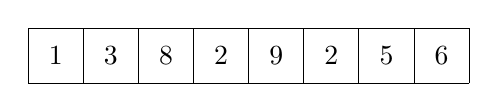
\begin{tikzpicture}[scale=0.7]
\draw (0,0) grid (8,1);
\node at (0.5,0.5) {$1$};
\node at (1.5,0.5) {$3$};
\node at (2.5,0.5) {$8$};
\node at (3.5,0.5) {$2$};
\node at (4.5,0.5) {$9$};
\node at (5.5,0.5) {$2$};
\node at (6.5,0.5) {$5$};
\node at (7.5,0.5) {$6$};
\end{tikzpicture}
\end{center}
quedará como sigue después de ordenar:
\begin{center}
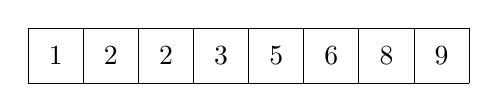
\begin{tikzpicture}[scale=0.7]
\draw (0,0) grid (8,1);
\node at (0.5,0.5) {$1$};
\node at (1.5,0.5) {$2$};
\node at (2.5,0.5) {$2$};
\node at (3.5,0.5) {$3$};
\node at (4.5,0.5) {$5$};
\node at (5.5,0.5) {$6$};
\node at (6.5,0.5) {$8$};
\node at (7.5,0.5) {$9$};
\end{tikzpicture}
\end{center}

\subsubsection{Algoritmos $O(n^2)$}

\index{ordenamiento de burbuja}

Los algoritmos sencillos para ordenar un arreglo
funcionan en tiempo $O(n^2)$.
Tales algoritmos son cortos y normalmente
constan de dos bucles anidados.
Un famoso algoritmo de ordenamiento de tiempo $O(n^2)$
es el \key{ordenamiento de burbuja}, donde los elementos
''burbujean'' en el arreglo según sus valores.

El ordenamiento de burbuja consta de $n$ rondas.
En cada ronda, el algoritmo recorre
los elementos del arreglo.
Siempre que se encuentran dos elementos consecutivos
que no están en el orden correcto,
el algoritmo los intercambia.
El algoritmo puede implementarse de la siguiente manera:
\begin{lstlisting}
for (int i = 0; i < n; i++) {
    for (int j = 0; j < n-1; j++) {
        if (array[j] > array[j+1]) {
            swap(array[j],array[j+1]);
        }
    }
}
\end{lstlisting}

Después de la primera ronda del algoritmo,
el elemento más grande estará en la posición correcta,
y en general, después de $k$ rondas, los $k$ elementos
más grandes estarán en las posiciones correctas.
Así, después de $n$ rondas, todo el arreglo
estará ordenado.

Por ejemplo, en el arreglo

\begin{center}
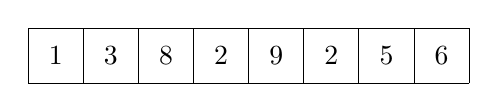
\begin{tikzpicture}[scale=0.7]
\draw (0,0) grid (8,1);

\node at (0.5,0.5) {$1$};
\node at (1.5,0.5) {$3$};
\node at (2.5,0.5) {$8$};
\node at (3.5,0.5) {$2$};
\node at (4.5,0.5) {$9$};
\node at (5.5,0.5) {$2$};
\node at (6.5,0.5) {$5$};
\node at (7.5,0.5) {$6$};
\end{tikzpicture}
\end{center}

\noindent
la primera ronda del ordenamiento de burbuja intercambia elementos
de la siguiente manera:

\begin{center}
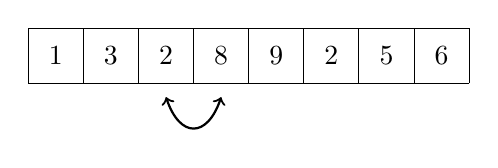
\begin{tikzpicture}[scale=0.7]
\draw (0,0) grid (8,1);
\node at (0.5,0.5) {$1$};
\node at (1.5,0.5) {$3$};
\node at (2.5,0.5) {$2$};
\node at (3.5,0.5) {$8$};
\node at (4.5,0.5) {$9$};
\node at (5.5,0.5) {$2$};
\node at (6.5,0.5) {$5$};
\node at (7.5,0.5) {$6$};

\draw[thick,<->] (3.5,-0.25) .. controls (3.25,-1.00) and (2.75,-1.00) .. (2.5,-0.25);
\end{tikzpicture}
\end{center}

\begin{center}
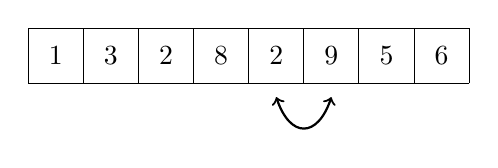
\begin{tikzpicture}[scale=0.7]
\draw (0,0) grid (8,1);
\node at (0.5,0.5) {$1$};
\node at (1.5,0.5) {$3$};
\node at (2.5,0.5) {$2$};
\node at (3.5,0.5) {$8$};
\node at (4.5,0.5) {$2$};
\node at (5.5,0.5) {$9$};
\node at (6.5,0.5) {$5$};
\node at (7.5,0.5) {$6$};

\draw[thick,<->] (5.5,-0.25) .. controls (5.25,-1.00) and (4.75,-1.00) .. (4.5,-0.25);
\end{tikzpicture}
\end{center}

\begin{center}
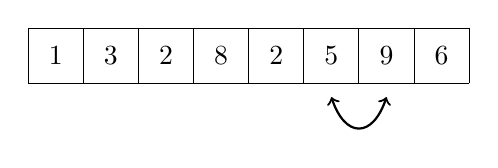
\begin{tikzpicture}[scale=0.7]
\draw (0,0) grid (8,1);
\node at (0.5,0.5) {$1$};
\node at (1.5,0.5) {$3$};
\node at (2.5,0.5) {$2$};
\node at (3.5,0.5) {$8$};
\node at (4.5,0.5) {$2$};
\node at (5.5,0.5) {$5$};
\node at (6.5,0.5) {$9$};
\node at (7.5,0.5) {$6$};

\draw[thick,<->] (6.5,-0.25) .. controls (6.25,-1.00) and (5.75,-1.00) .. (5.5,-0.25);
\end{tikzpicture}
\end{center}

\begin{center}
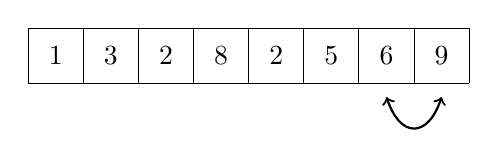
\begin{tikzpicture}[scale=0.7]
\draw (0,0) grid (8,1);
\node at (0.5,0.5) {$1$};
\node at (1.5,0.5) {$3$};
\node at (2.5,0.5) {$2$};
\node at (3.5,0.5) {$8$};
\node at (4.5,0.5) {$2$};
\node at (5.5,0.5) {$5$};
\node at (6.5,0.5) {$6$};
\node at (7.5,0.5) {$9$};

\draw[thick,<->] (7.5,-0.25) .. controls (7.25,-1.00) and (6.75,-1.00) .. (6.5,-0.25);
\end{tikzpicture}
\end{center}

\subsubsection{Inversiones}

\index{inversión}

El ordenamiento de burbuja es un ejemplo de un algoritmo
de ordenamiento que siempre intercambia elementos
\emph{consecutivos} del arreglo.
Resulta que la complejidad temporal
de tal algoritmo es \emph{siempre}
al menos $O(n^2)$, porque en el peor caso,
se requieren $O(n^2)$ intercambios para ordenar el arreglo.

Un concepto útil al analizar algoritmos
de ordenamiento es una \key{inversión}:
un par de elementos del arreglo
$(\texttt{array}[a],\texttt{array}[b])$ tal que
$a<b$ y $\texttt{array}[a]>\texttt{array}[b]$,
es decir, los elementos están en el orden incorrecto.
Por ejemplo, el arreglo
\begin{center}
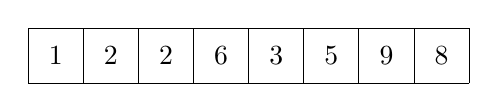
\begin{tikzpicture}[scale=0.7]
\draw (0,0) grid (8,1);
\node at (0.5,0.5) {$1$};
\node at (1.5,0.5) {$2$};
\node at (2.5,0.5) {$2$};
\node at (3.5,0.5) {$6$};
\node at (4.5,0.5) {$3$};
\node at (5.5,0.5) {$5$};
\node at (6.5,0.5) {$9$};
\node at (7.5,0.5) {$8$};
\end{tikzpicture}
\end{center}
tiene tres inversiones: $(6,3)$, $(6,5)$ y $(9,8)$.
El número de inversiones indica
cuánto trabajo se necesita para ordenar el arreglo.
Un arreglo está completamente ordenado cuando
no hay inversiones.
Por otro lado, si los elementos del arreglo
están en el orden inverso,
el número de inversiones es el mayor posible:
\[1+2+\cdots+(n-1)=\frac{n(n-1)}{2} = O(n^2)\]

Intercambiar un par de elementos consecutivos que están
en el orden incorrecto elimina exactamente una inversión
del arreglo.
Por lo tanto, si un algoritmo de ordenamiento solo puede
intercambiar elementos consecutivos, cada intercambio elimina
a lo sumo una inversión, y la complejidad temporal
del algoritmo es al menos $O(n^2)$.

\subsubsection{Algoritmos $O(n \log n)$}

\index{ordenamiento por mezcla}

Es posible ordenar un arreglo de forma eficiente
en tiempo $O(n \log n)$ usando algoritmos
que no se limitan a intercambiar elementos consecutivos.
Uno de tales algoritmos es el \key{ordenamiento por mezcla}\footnote{Según \cite{knu983},
el ordenamiento por mezcla fue inventado por J. von Neumann en 1945.},
que se basa en la recursión.

El ordenamiento por mezcla ordena un subarreglo \texttt{array}$[a \ldots b]$ de la siguiente manera:

\begin{enumerate}
\item Si $a=b$, no hagas nada, porque el subarreglo ya está ordenado.
\item Calcula la posición del elemento del medio: $k=\lfloor (a+b)/2 \rfloor$.
\item Ordena recursivamente el subarreglo \texttt{array}$[a \ldots k]$.
\item Ordena recursivamente el subarreglo \texttt{array}$[k+1 \ldots b]$.
\item \emph{Mezcla} los subarreglos ordenados \texttt{array}$[a \ldots k]$ y
\texttt{array}$[k+1 \ldots b]$
en un subarreglo ordenado \texttt{array}$[a \ldots b]$.
\end{enumerate}

El ordenamiento por mezcla es un algoritmo eficiente, porque
reduce a la mitad el tamaño del subarreglo en cada paso.
La recursión consta de $O(\log n)$ niveles,
y procesar cada nivel toma $O(n)$ de tiempo.
Mezclar los subarreglos \texttt{array}$[a \ldots k]$ y \texttt{array}$[k+1 \ldots b]$
es posible en tiempo lineal, porque ya están ordenados.

Por ejemplo, considera ordenar el siguiente arreglo:
\begin{center}
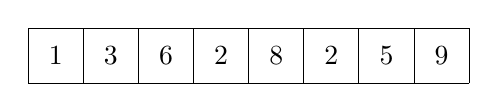
\begin{tikzpicture}[scale=0.7]
\draw (0,0) grid (8,1);
\node at (0.5,0.5) {$1$};
\node at (1.5,0.5) {$3$};
\node at (2.5,0.5) {$6$};
\node at (3.5,0.5) {$2$};
\node at (4.5,0.5) {$8$};
\node at (5.5,0.5) {$2$};
\node at (6.5,0.5) {$5$};
\node at (7.5,0.5) {$9$};
\end{tikzpicture}
\end{center}

El arreglo se dividirá en dos subarreglos
de la siguiente manera:
\begin{center}
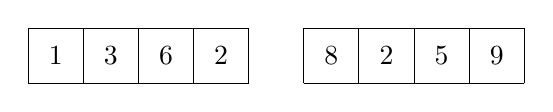
\begin{tikzpicture}[scale=0.7]
\draw (0,0) grid (4,1);
\draw (5,0) grid (9,1);

\node at (0.5,0.5) {$1$};
\node at (1.5,0.5) {$3$};
\node at (2.5,0.5) {$6$};
\node at (3.5,0.5) {$2$};

\node at (5.5,0.5) {$8$};
\node at (6.5,0.5) {$2$};
\node at (7.5,0.5) {$5$};
\node at (8.5,0.5) {$9$};
\end{tikzpicture}
\end{center}

Luego, los subarreglos se ordenarán recursivamente
de la siguiente manera:
\begin{center}
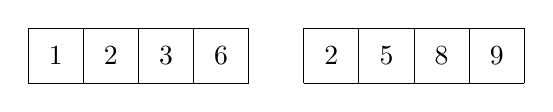
\begin{tikzpicture}[scale=0.7]
\draw (0,0) grid (4,1);
\draw (5,0) grid (9,1);

\node at (0.5,0.5) {$1$};
\node at (1.5,0.5) {$2$};
\node at (2.5,0.5) {$3$};
\node at (3.5,0.5) {$6$};

\node at (5.5,0.5) {$2$};
\node at (6.5,0.5) {$5$};
\node at (7.5,0.5) {$8$};
\node at (8.5,0.5) {$9$};
\end{tikzpicture}
\end{center}

Finalmente, el algoritmo mezcla los subarreglos
ordenados y crea el arreglo ordenado final:
\begin{center}
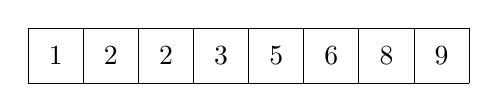
\begin{tikzpicture}[scale=0.7]
\draw (0,0) grid (8,1);
\node at (0.5,0.5) {$1$};
\node at (1.5,0.5) {$2$};
\node at (2.5,0.5) {$2$};
\node at (3.5,0.5) {$3$};
\node at (4.5,0.5) {$5$};
\node at (5.5,0.5) {$6$};
\node at (6.5,0.5) {$8$};
\node at (7.5,0.5) {$9$};
\end{tikzpicture}
\end{center}

\subsubsection{Cota inferior del ordenamiento}

¿Es posible ordenar un arreglo más rápido
que en tiempo $O(n \log n)$?
Resulta que esto \emph{no} es posible
cuando nos restringimos a algoritmos de ordenamiento
que se basan en comparar elementos del arreglo.

La cota inferior de la complejidad temporal
puede demostrarse considerando el ordenamiento
como un proceso donde cada comparación de dos elementos
da más información sobre el contenido del arreglo.
El proceso crea el siguiente árbol:

\begin{center}
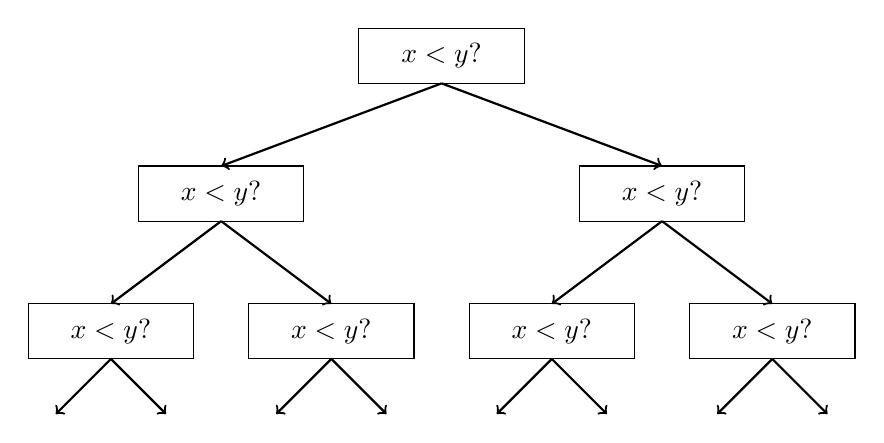
\begin{tikzpicture}[scale=0.7]
\draw (0,0) rectangle (3,1);
\node at (1.5,0.5) {$x < y?$};

\draw[thick,->] (1.5,0) -- (-2.5,-1.5);
\draw[thick,->] (1.5,0) -- (5.5,-1.5);

\draw (-4,-2.5) rectangle (-1,-1.5);
\draw (4,-2.5) rectangle (7,-1.5);
\node at (-2.5,-2) {$x < y?$};
\node at (5.5,-2) {$x < y?$};

\draw[thick,->] (-2.5,-2.5) -- (-4.5,-4);
\draw[thick,->] (-2.5,-2.5) -- (-0.5,-4);
\draw[thick,->] (5.5,-2.5) -- (3.5,-4);
\draw[thick,->] (5.5,-2.5) -- (7.5,-4);

\draw (-6,-5) rectangle (-3,-4);
\draw (-2,-5) rectangle (1,-4);
\draw (2,-5) rectangle (5,-4);
\draw (6,-5) rectangle (9,-4);
\node at (-4.5,-4.5) {$x < y?$};
\node at (-0.5,-4.5) {$x < y?$};
\node at (3.5,-4.5) {$x < y?$};
\node at (7.5,-4.5) {$x < y?$};

\draw[thick,->] (-4.5,-5) -- (-5.5,-6);
\draw[thick,->] (-4.5,-5) -- (-3.5,-6);
\draw[thick,->] (-0.5,-5) -- (0.5,-6);
\draw[thick,->] (-0.5,-5) -- (-1.5,-6);
\draw[thick,->] (3.5,-5) -- (2.5,-6);
\draw[thick,->] (3.5,-5) -- (4.5,-6);
\draw[thick,->] (7.5,-5) -- (6.5,-6);
\draw[thick,->] (7.5,-5) -- (8.5,-6);
\end{tikzpicture}
\end{center}

Aquí ''$x<y?$'' significa que se comparan algunos elementos
$x$ y $y$.
Si $x<y$, el proceso continúa hacia la izquierda,
y en caso contrario hacia la derecha.
Los resultados del proceso son las posibles
formas de ordenar el arreglo, un total de $n!$ formas.
Por esta razón, la altura del árbol
debe ser al menos
\[ \log_2(n!) = \log_2(1)+\log_2(2)+\cdots+\log_2(n).\]
Obtenemos una cota inferior para esta suma
eligiendo los últimos $n/2$ elementos y
cambiando el valor de cada elemento a $\log_2(n/2)$.
Esto produce una estimación
\[ \log_2(n!) \ge (n/2) \cdot \log_2(n/2),\]
así que la altura del árbol y el número mínimo
posible de pasos en un algoritmo de
ordenamiento en el peor caso
es al menos $n \log n$.

\subsubsection{Ordenamiento por conteo}

\index{ordenamiento por conteo}

La cota inferior $n \log n$ no se aplica a
algoritmos que no comparan elementos del arreglo
sino que usan alguna otra información.
Un ejemplo de tal algoritmo es
el \key{ordenamiento por conteo}, que ordena un arreglo en
tiempo $O(n)$ suponiendo que todo elemento del arreglo
es un entero entre $0 \ldots c$ y $c=O(n)$.

El algoritmo crea un arreglo de \emph{conteo},
cuyos índices son los elementos del arreglo original.
El algoritmo recorre el arreglo original
y calcula cuántas veces aparece cada elemento
en el arreglo.
\newpage

Por ejemplo, el arreglo
\begin{center}
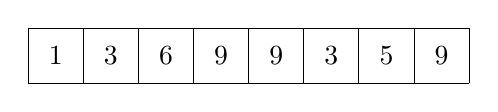
\begin{tikzpicture}[scale=0.7]
\draw (0,0) grid (8,1);
\node at (0.5,0.5) {$1$};
\node at (1.5,0.5) {$3$};
\node at (2.5,0.5) {$6$};
\node at (3.5,0.5) {$9$};
\node at (4.5,0.5) {$9$};
\node at (5.5,0.5) {$3$};
\node at (6.5,0.5) {$5$};
\node at (7.5,0.5) {$9$};
\end{tikzpicture}
\end{center}
corresponde al siguiente arreglo de conteo:
\begin{center}
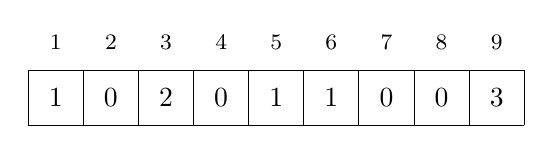
\begin{tikzpicture}[scale=0.7]
\draw (0,0) grid (9,1);
\node at (0.5,0.5) {$1$};
\node at (1.5,0.5) {$0$};
\node at (2.5,0.5) {$2$};
\node at (3.5,0.5) {$0$};
\node at (4.5,0.5) {$1$};
\node at (5.5,0.5) {$1$};
\node at (6.5,0.5) {$0$};
\node at (7.5,0.5) {$0$};
\node at (8.5,0.5) {$3$};

\footnotesize

\node at (0.5,1.5) {$1$};
\node at (1.5,1.5) {$2$};
\node at (2.5,1.5) {$3$};
\node at (3.5,1.5) {$4$};
\node at (4.5,1.5) {$5$};
\node at (5.5,1.5) {$6$};
\node at (6.5,1.5) {$7$};
\node at (7.5,1.5) {$8$};
\node at (8.5,1.5) {$9$};
\end{tikzpicture}
\end{center}

Por ejemplo, el valor en la posición 3
del arreglo de conteo es 2,
porque el elemento 3 aparece 2 veces
en el arreglo original.

La construcción del arreglo de conteo
toma $O(n)$ de tiempo. Después de esto, el arreglo ordenado
puede crearse en tiempo $O(n)$ porque
el número de apariciones de cada elemento puede recuperarse
del arreglo de conteo.
Así, la complejidad temporal total del ordenamiento
por conteo es $O(n)$.

El ordenamiento por conteo es un algoritmo muy eficiente
pero solo puede usarse cuando la constante $c$
es lo bastante pequeña, de modo que los elementos del arreglo puedan
usarse como índices en el arreglo de conteo.

\section{Ordenamiento en C++}

\index{sort@\texttt{sort}}

Casi nunca es buena idea usar
un algoritmo de ordenamiento hecho en casa
en un concurso, porque hay buenas
implementaciones disponibles en los lenguajes de programación.
Por ejemplo, la biblioteca estándar de C++ contiene
la función \texttt{sort} que puede usarse fácilmente para
ordenar arreglos y otras estructuras de datos.

Usar una función de biblioteca tiene muchos beneficios.
Primero, ahorra tiempo porque no hay necesidad de
implementar la función.
Segundo, la implementación de la biblioteca es
sin duda correcta y eficiente: no es probable
que una función de ordenamiento hecha en casa sea mejor.

En esta sección veremos cómo usar la
función \texttt{sort} de C++.
El siguiente código ordena
un vector en orden creciente:
\begin{lstlisting}
vector<int> v = {4,2,5,3,5,8,3};
sort(v.begin(),v.end());
\end{lstlisting}
Después del ordenamiento, el contenido del
vector será
$[2,3,3,4,5,5,8]$.
El orden de ordenamiento por defecto es creciente,
pero un orden inverso es posible de la siguiente manera:
\begin{lstlisting}
sort(v.rbegin(),v.rend());
\end{lstlisting}
Un arreglo ordinario puede ordenarse de la siguiente manera:
\begin{lstlisting}
int n = 7; // array size
int a[] = {4,2,5,3,5,8,3};
sort(a,a+n);
\end{lstlisting}
\newpage
El siguiente código ordena la cadena \texttt{s}:
\begin{lstlisting}
string s = "monkey";
sort(s.begin(), s.end());
\end{lstlisting}
Ordenar una cadena significa que los caracteres
de la cadena se ordenan.
Por ejemplo, la cadena ''monkey'' se convierte en ''ekmnoy''.

\subsubsection{Operadores de comparación}

\index{operador de comparación}

La función \texttt{sort} requiere que
se defina un \key{operador de comparación} para el tipo de dato
de los elementos que se van a ordenar.
Al ordenar, este operador se usará
siempre que sea necesario averiguar el orden de dos elementos.

La mayoría de los tipos de datos de C++ tienen un operador de comparación integrado,
y los elementos de esos tipos pueden ordenarse automáticamente.
Por ejemplo, los números se ordenan según sus valores
y las cadenas se ordenan en orden alfabético.

\index{pair@\texttt{pair}}

Los pares (\texttt{pair}) se ordenan principalmente según sus
primeros elementos (\texttt{first}).
Sin embargo, si los primeros elementos de dos pares son iguales,
se ordenan según sus segundos elementos (\texttt{second}):
\begin{lstlisting}
vector<pair<int,int>> v;
v.push_back({1,5});
v.push_back({2,3});
v.push_back({1,2});
sort(v.begin(), v.end());
\end{lstlisting}
Después de esto, el orden de los pares es
$(1,2)$, $(1,5)$ y $(2,3)$.

\index{tuple@\texttt{tuple}}

De manera similar, las tuplas (\texttt{tuple})
se ordenan principalmente por el primer elemento,
secundariamente por el segundo elemento, etc.\footnote{Nota que en algunos compiladores más antiguos,
hay que usar la función \texttt{make\_tuple} para crear una tupla en lugar de
llaves (por ejemplo, \texttt{make\_tuple(2,1,4)} en vez de \texttt{\{2,1,4\}}).}:
\begin{lstlisting}
vector<tuple<int,int,int>> v;
v.push_back({2,1,4});
v.push_back({1,5,3});
v.push_back({2,1,3});
sort(v.begin(), v.end());
\end{lstlisting}
Después de esto, el orden de las tuplas es
$(1,5,3)$, $(2,1,3)$ y $(2,1,4)$.

\subsubsection{Structs definidos por el usuario}

Los structs definidos por el usuario no tienen un operador
de comparación automáticamente.
El operador debe definirse dentro
del struct como una función
\texttt{operator<},
cuyo parámetro es otro elemento del mismo tipo.
El operador debe devolver \texttt{true}
si el elemento es menor que el parámetro,
y \texttt{false} en caso contrario.

Por ejemplo, el siguiente struct \texttt{P}
contiene las coordenadas x e y de un punto.
El operador de comparación se define de modo que
los puntos se ordenen principalmente por la coordenada x
y secundariamente por la coordenada y.

\begin{lstlisting}
struct P {
    int x, y;
    bool operator<(const P &p) {
        if (x != p.x) return x < p.x;
        else return y < p.y;
    }
};
\end{lstlisting}

\subsubsection{Funciones de comparación}

\index{función de comparación}

También es posible dar una \key{función de comparación}
externa a la función \texttt{sort}
como una función de retorno (callback).
Por ejemplo, la siguiente función de comparación \texttt{comp}
ordena cadenas principalmente por longitud y secundariamente
por orden alfabético:

\begin{lstlisting}
bool comp(string a, string b) {
    if (a.size() != b.size()) return a.size() < b.size();
    return a < b;
}
\end{lstlisting}
Ahora un vector de cadenas puede ordenarse de la siguiente manera:
\begin{lstlisting}
sort(v.begin(), v.end(), comp);
\end{lstlisting}

\section{Búsqueda binaria}

\index{búsqueda binaria}

Un método general para buscar un elemento
en un arreglo es usar un bucle \texttt{for}
que recorra los elementos del arreglo.
Por ejemplo, el siguiente código busca
un elemento $x$ en un arreglo:

\begin{lstlisting}
for (int i = 0; i < n; i++) {
    if (array[i] == x) {
        // x found at index i
    }
}
\end{lstlisting}

La complejidad temporal de este enfoque es $O(n)$,
porque en el peor caso, es necesario revisar
todos los elementos del arreglo.
Si el orden de los elementos es arbitrario,
este es también el mejor enfoque posible, porque
no hay información adicional disponible sobre en qué parte
del arreglo deberíamos buscar el elemento $x$.

Sin embargo, si el arreglo está \emph{ordenado},
la situación es distinta.
En este caso es posible realizar la
búsqueda mucho más rápido, porque el orden de los
elementos del arreglo guía la búsqueda.
El siguiente algoritmo de \key{búsqueda binaria}
busca eficientemente un elemento en un arreglo ordenado
en tiempo $O(\log n)$.

\subsubsection{Método 1}

La forma habitual de implementar la búsqueda binaria
se asemeja a buscar una palabra en un diccionario.
La búsqueda mantiene una región activa en el arreglo,
que inicialmente contiene todos los elementos del arreglo.
Luego, se realiza una serie de pasos,
cada uno de los cuales reduce a la mitad el tamaño de la región.

En cada paso, la búsqueda revisa el elemento del medio
de la región activa.
Si el elemento del medio es el elemento buscado,
la búsqueda termina.
En caso contrario, la búsqueda continúa recursivamente
hacia la mitad izquierda o derecha de la región,
según el valor del elemento del medio.

La idea anterior puede implementarse de la siguiente manera:
\begin{lstlisting}
int a = 0, b = n-1;
while (a <= b) {
    int k = (a+b)/2;
    if (array[k] == x) {
        // x found at index k
    }
    if (array[k] > x) b = k-1;
    else a = k+1;
}
\end{lstlisting}

En esta implementación, la región activa es $a \ldots b$,
e inicialmente la región es $0 \ldots n-1$.
El algoritmo reduce a la mitad el tamaño de la región en cada paso,
así que la complejidad temporal es $O(\log n)$.

\subsubsection{Método 2}

Un método alternativo para implementar la búsqueda binaria
se basa en una forma eficiente de recorrer
los elementos del arreglo.
La idea es hacer saltos y reducir la velocidad
cuando nos acercamos al elemento buscado.

La búsqueda recorre el arreglo de izquierda a
derecha, y la longitud inicial del salto es $n/2$.
En cada paso, la longitud del salto se reduce a la mitad:
primero $n/4$, luego $n/8$, $n/16$, etc., hasta que
finalmente la longitud es 1.
Después de los saltos, o bien se ha encontrado el elemento
buscado o sabemos que no aparece en el arreglo.

El siguiente código implementa la idea anterior:
\begin{lstlisting}
int k = 0;
for (int b = n/2; b >= 1; b /= 2) {
    while (k+b < n && array[k+b] <= x) k += b;
}
if (array[k] == x) {
    // x found at index k
}
\end{lstlisting}

Durante la búsqueda, la variable $b$
contiene la longitud actual del salto.
La complejidad temporal del algoritmo es $O(\log n)$,
porque el código del bucle \texttt{while}
se ejecuta a lo sumo dos veces por cada longitud de salto.

\subsubsection{Funciones de C++}

La biblioteca estándar de C++ contiene las siguientes funciones
que se basan en la búsqueda binaria y funcionan en tiempo logarítmico:

\begin{itemize}
\item \texttt{lower\_bound} devuelve un puntero al
primer elemento del arreglo cuyo valor es al menos $x$.
\item \texttt{upper\_bound} devuelve un puntero al
primer elemento del arreglo cuyo valor es mayor que $x$.
\item \texttt{equal\_range} devuelve ambos punteros anteriores.
\end{itemize}

Las funciones suponen que el arreglo está ordenado.
Si no existe tal elemento, el puntero apunta
al elemento posterior al último elemento del arreglo.
Por ejemplo, el siguiente código averigua si
un arreglo contiene un elemento con valor $x$:

\begin{lstlisting}
auto k = lower_bound(array,array+n,x)-array;
if (k < n && array[k] == x) {
    // x found at index k
}
\end{lstlisting}

Luego, el siguiente código cuenta el número de elementos
cuyo valor es $x$:

\begin{lstlisting}
auto a = lower_bound(array, array+n, x);
auto b = upper_bound(array, array+n, x);
cout << b-a << "\n";
\end{lstlisting}

Usando \texttt{equal\_range}, el código se vuelve más corto:

\begin{lstlisting}
auto r = equal_range(array, array+n, x);
cout << r.second-r.first << "\n";
\end{lstlisting}

\subsubsection{Encontrar la solución más pequeña}

Un uso importante de la búsqueda binaria es
encontrar la posición donde cambia el valor de una \emph{función}.
Supongamos que deseamos encontrar el valor más pequeño $k$
que es una solución válida para un problema.
Se nos da una función $\texttt{ok}(x)$
que devuelve \texttt{true} si $x$ es una solución válida
y \texttt{false} en caso contrario.
Además, sabemos que $\texttt{ok}(x)$ es \texttt{false}
cuando $x<k$ y \texttt{true} cuando $x \ge k$.
La situación se ve de la siguiente manera:

\begin{center}
\begin{tabular}{r|rrrrrrrr}
$x$ & 0 & 1 & $\cdots$ & $k-1$ & $k$ & $k+1$ & $\cdots$ \\
\hline
$\texttt{ok}(x)$ & \texttt{false} & \texttt{false}
& $\cdots$ & \texttt{false} & \texttt{true} & \texttt{true} & $\cdots$ \\
\end{tabular}
\end{center}

\noindent
Ahora, el valor de $k$ puede encontrarse usando búsqueda binaria:

\begin{lstlisting}
int x = -1;
for (int b = z; b >= 1; b /= 2) {
    while (!ok(x+b)) x += b;
}
int k = x+1;
\end{lstlisting}

La búsqueda encuentra el mayor valor de $x$ para el cual
$\texttt{ok}(x)$ es \texttt{false}.
Así, el siguiente valor $k=x+1$
es el menor valor posible para el cual
$\texttt{ok}(k)$ es \texttt{true}.
La longitud inicial del salto $z$ tiene que ser
lo bastante grande, por ejemplo algún valor
para el cual sepamos de antemano que $\texttt{ok}(z)$ es \texttt{true}.

El algoritmo llama a la función \texttt{ok}
$O(\log z)$ veces, así que la complejidad temporal total
depende de la función \texttt{ok}.
Por ejemplo, si la función funciona en tiempo $O(n)$,
la complejidad temporal total es $O(n \log z)$.

\subsubsection{Encontrar el valor máximo}

La búsqueda binaria también puede usarse para encontrar
el valor máximo de una función que es
primero creciente y luego decreciente.
Nuestra tarea es encontrar una posición $k$ tal que

\begin{itemize}
\item
$f(x)<f(x+1)$ cuando $x<k$, y
\item
$f(x)>f(x+1)$ cuando $x \ge k$.
\end{itemize}

La idea es usar búsqueda binaria
para encontrar el mayor valor de $x$
para el cual $f(x)<f(x+1)$.
Esto implica que $k=x+1$
porque $f(x+1)>f(x+2)$.
El siguiente código implementa la búsqueda:

\begin{lstlisting}
int x = -1;
for (int b = z; b >= 1; b /= 2) {
    while (f(x+b) < f(x+b+1)) x += b;
}
int k = x+1;
\end{lstlisting}

Nota que a diferencia de la búsqueda binaria ordinaria,
aquí no se permite que valores consecutivos
de la función sean iguales.
En ese caso no sería posible saber
cómo continuar la búsqueda.
